% CLASS 2 -- the notes' section 1.2, sec.messageFiles.
% Budget 60 min of slides, then the two notebooks; planned 66 over 16 frames.
% Overrunning, cut in this order: the consolidated tape (Regulation NMS is background and
% plays no part in the assignment), then the nomenclature frame (the vendor names survive as
% the sentence under the schematic), then hand the termination argument to the notebook.
% That lands at 60.
%
% LABELS. The five class files are \include'd into ONE document, so a label is defined once
% across all five, and a cross-file \ref prints ?? on a clean tree. These are class 2's:
% remark.whyReconstruct, remark.derivedAndDelayed, remark.aggregatedAsCheck, eq.bookFold,
% remark.gridAgainstOccupied, remark.passiveDirection.
% Class 1 owns def.orderQueue, prop.lobUpdate, prop.decompositionOfLimitOrder and
% eq.queueImbalance; each is RESTATED HERE WITHOUT A LABEL, in one line, and none is \ref'd.
% Section numbers of the notes are written out as digits, as class 1 writes them.
%
% algo.bookFold appears on its own frame as a bare `algorithmic' environment: `algorithm' is
% a float and floats do not place inside a frame, so there is no caption, no line numbering
% and no \label{algo.*} here.
%
% A frame holds 218pt of body -- eighteen 12pt lines, or seven two-line paragraphs.

\subsection{From message files to the aggregated order book}

\begin{frame}
  \frametitle{Outline}
% One \nocite per line -- a multi-key \nocite spanning lines breaks bibtex.
\nocite{HP11lob}
\nocite{DBG24eob}
\nocite{NAS23itc}
\nocite{LPV22sho}
Section 1.1 described a limit order book at one instant.
This class is about where those instants come from,
and about why a participant computes them rather than receiving them.

\pause

An exchange publishes the same events twice,
once as a stream of orders and once as a book of totals,
and the second is a function of the first.
We say what that function discards,
and what it costs to be handed its output rather than to apply it oneself.

\pause

We then write the book as a fold,
and read the two files LOBSTER distributes as the recorded form of the same pair.
Section 1.4 computes its statistics from exactly these files.
\end{frame}

\begin{frame}
  \frametitle{A matching engine publishes two views of one truth}
\begin{center}
\begin{tikzpicture}[font=\scriptsize,
    box/.style={draw=gray!70, rounded corners=2pt, align=center, inner sep=3pt}]
  \node[box, fill=gray!15] (engine) at (0,0) {matching\\engine};
  \node[box, fill=blue!15, text width=2.9cm] (stream) at (4.8,0.82)
       {\emph{message stream}\\one message per order event};
  \node[box, fill=orange!30] (agg) at (2.5,-0.82) {aggregation};
  \node[box, fill=orange!15, text width=2.9cm] (level) at (5.8,-0.82)
       {\emph{aggregated book}\\total size at each of $L$ prices};
  \draw[-{Stealth}, gray!70] (engine.north east) -- (stream.west);
  \draw[-{Stealth}, gray!70] (engine.south east) -- (agg.west);
  \draw[-{Stealth}, gray!70] (agg.east) -- (level.west);
\end{tikzpicture}
\end{center}
The message stream carries one message per submission, cancellation, deletion and execution,
each naming the order it concerns;
it is the tape of the orders themselves,
and the trading epoch of Section 1.1 is exactly what it transmits.

\pause

The aggregated book carries the size resting at each of the first $L$ levels of each side,
republished as it changes:
the configuration of Section 1.1, truncated at depth $L$.
\end{frame}

\begin{frame}
  \frametitle{The aggregate is the image of the stream}
The two are not independent products.
The queues $\askOrderQueue_t$ and $\bidOrderQueue_t$ are sets of orders,
and the sizes $\nthBestAskSize[i]_t$ and $\nthBestBidSize[i]_t$ are sums over them,
so the second stream is the image of the first under those sums.

\pause

The exchange computes that image by applying the matching rules of Section 1.1 to its own
message stream,
which is to say that it runs the fold we write next before publishing the result.

\pause

A sum does not record its summands:
the aggregate says how much rests at a price,
never how that size is split between orders,
nor which of them the matching algorithm reaches first.

\pause

\begin{remark}
\label{remark.whyReconstruct}
 The aggregated book retains the quantity this chapter is about:
 how size has accumulated across the price levels of the two sides.
 That cross-section is what the queue imbalance $\queueImbalance[n]$ and the order flow
 imbalance of Section 1.4 are computed from.
\end{remark}
\end{frame}

\begin{frame}
  \frametitle{The aggregation sits in the publication path}
\begin{remark}
\label{remark.derivedAndDelayed}
 Notice that the aggregated book is derived, and that the derivation sits in the
 publication path:
 a message is on the wire once the engine has written it,
 whereas a level update exists only once the event has been netted against the level's
 total.
 The aggregation is left out of the message stream by design,
 price levels and their aggregation being derivable by the recipient from the individual
 orders, and the stream being published
 ``in order to send public market data as fast as possible''
 \cite[Section 3.1]{DBG24eob}.
\end{remark}

\pause

A participant who folds the stream herself therefore holds the aggregated book sooner,
and to a depth the feed does not publish.

\pause

The wire is not what separates them.
Both feeds are fixed-length binary on the same transport;
what differs is how many stages of the venue's own book-building sit between the match and
the message.
\end{frame}

\begin{frame}
  \frametitle{Truncation and netting remove states, not just time}
The aggregated book is truncated at depth $L$,
and where the feed is netted its updates are sent at regular intervals,
so that intermediate configurations are absent rather than delayed.

\pause

A level whose total is unchanged publishes nothing.
Ten orders resting at the best bid, one of them added and another partly filled between two
intervals, can leave the level's total where it was,
and the aggregated feed is then silent about both events.

\pause

Limited-depth products go further and restate the book with each snapshot rather than sending
incremental deltas \cite{CME26mbl},
so the configurations between two snapshots are not recoverable at any latency.

\pause

Waiting longer recovers a delayed state.
No amount of waiting recovers one that was never published.
\end{frame}

\begin{frame}
  \frametitle{Queue position is recoverable only from the order stream}
A message carries the identity of the order it concerns,
so a participant folding the stream knows how many shares rest ahead of her own order at its
price, and in what order they will be reached.

\pause

The aggregate carries only the total.
The split it discards is what decides whether a given resting order is executed,
and Section 1.1 sets that split aside.

\pause

Fill probability is a function of the discarded split,
and no latency buys it back:
a participant may read the aggregated feed arbitrarily early and still not know her place in
the queue.
\end{frame}

\begin{frame}
  \frametitle{The nomenclature is not standardised}
Both products are shipped on every major venue.
Eurex publishes the message stream as the Enhanced Order Book Interface,
and the aggregated book twice over:
as the Enhanced Market Data Interface, un-netted,
and as the Market Data Interface, whose updates are netted at regular intervals
\cite{DBG24eob, DBG24emd}.

\pause

On CME's MDP 3.0 the same event appears in a market-by-order and in a market-by-price book
\cite{CMEmdp, CME26mbo},
and Nasdaq publishes the message stream as TotalView-ITCH \cite{NAS23itc, NAS26tot}.

\pause

Venues and vendors call the first of the two market by order, order by order or level three,
and the second market by price, depth of book or level two.
The three names on either line are one product.
\end{frame}

\begin{frame}
  \frametitle{A check, not a substitute}
\begin{remark}
\label{remark.aggregatedAsCheck}
 The two feeds have different jobs.
 A fold run on the message stream is the participant's own computation:
 it is available sooner and to any depth,
 and a dropped message or a mishandled event leaves it wrong
 in a way that no statistic computed from it reveals.
 The aggregated book is the exchange's own fold of the same stream,
 published later and truncated,
 and comparing the two level by level locates such an error where nothing else does.
 It is a check on the reconstruction rather than a substitute for it.
\end{remark}

\pause

A book that has drifted by one dropped message still has a mid-price, a spread and an
imbalance, all of them in range and all of them wrong.
The habit this asks for is two routes to one number,
with the disagreement read as a location rather than as a nuisance.
\end{frame}

\begin{frame}
  \frametitle{Consolidation costs a latency the venue's own feed does not}
A second tape exists in United States equities for a regulatory rather than a technical
reason.

\pause

Rule 603(c) of Regulation NMS obliges anyone who displays quotations,
where a trading decision can be implemented,
to display consolidated data alongside them \cite{SEC05reg}.

\pause

Consolidation is performed by a party other than the venue on which the quotation arose,
and costs a latency that a participant reading each venue's own feed does not pay.
\end{frame}

\begin{frame}
  \frametitle{The book is a fold, and holds one state}
Writing $\mathcal{B}$ for a configuration and $m_k$ for the $k$-th message of the stream,
\begin{equation}
\label{eq.bookFold}
 \mathcal{B}_{k} = F(\mathcal{B}_{k-1}, m_k),
 \qquad \mathcal{B}_0 = \varnothing ,
\end{equation}
so that the book is the accumulator of a fold and holds one state, the current one.

\pause

The sequence $(\mathcal{B}_k)_k$ is not held by the book;
it is produced by whatever drives the fold, at whatever resolution is wanted.

\pause

Sampling every message, every second, or only at the times a statistic is evaluated,
are three drivers of one accumulator,
and none of them is a different book.
\end{frame}

\begin{frame}
  \frametitle{The transition is one function, not a case analysis}
The transition $F$ is the update rule of Section 1.1:
the arrival of an order takes the aggregated state to the aggregated state,
with no reference to the individual orders resting behind the sizes.

\pause

What makes it a single function rather than a case analysis is the decomposition of
Section 1.1:
every incoming order is processed as its market part followed by its resting part.
There is no separate branch for a marketable order,
and an implementation that writes one has two code paths where the mathematics has one.

\pause

A message is a submission, carrying an order $(t,q,p,d)$,
or a cancellation, withdrawing a size $q$ from the queue at $p$ on the side $d$;
a deletion is the cancellation of all of it.

\pause

An execution is not a third kind:
it is the record of the market part of somebody else's submission,
read on the passive side.
\end{frame}

\begin{frame}
  \frametitle{Each pass of the loop empties one price}
{\footnotesize
\begin{algorithmic}
 \REQUIRE $\mathcal{B}_{k-1}$ as two maps from price to size, and the message $m_k$
 \IF{$m_k$ is a cancellation of $q$ at $p$ on the side $d$}
 \STATE subtract $q$ from the size at $p$ on the side $d$, and remove $p$ if it reaches zero
 \ELSE
 \STATE let $(t,q,p,d)$ be the submitted order and set its market part
        $\marketOrderSize$ by the decomposition
 \STATE set $r := \marketOrderSize$
 \WHILE{$r > 0$}
 \STATE let $\pi$ be the best price-eligible price on the side $-d$
 \STATE match $r \wedge \nthBestAskSize[1]$ shares at $\pi$ if $d=+1$, and
        $r \wedge \nthBestBidSize[1]$ if $d=-1$
 \STATE subtract them at $\pi$, remove $\pi$ if it reaches zero,
        and decrease $r$ by the same amount
 \ENDWHILE
 \STATE add $q - \marketOrderSize$ to the size at $p$ on the side $d$
 \ENDIF
 \RETURN $\mathcal{B}_{k}$
\end{algorithmic}
}

\pause

The loop is the reduction of the update rule to its elementary pieces,
and it terminates because each pass empties one price.
We implement it more than once,
and compare the implementations on the time and the memory they take.
\end{frame}

\begin{frame}
  \frametitle{A feed reports occupied prices, not grid levels}
\begin{center}
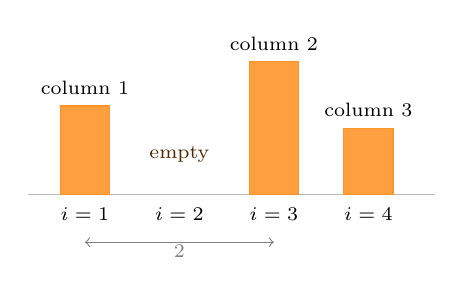
\begin{tikzpicture}[x=1.2cm, y=0.0094cm, font=\scriptsize]
  \draw[gray!55] (0.4,0) -- (4.7,0);
  \foreach \x/\h in {1/120, 3/180, 4/90}
    \draw[fill=orange!75, draw=orange!85] (\x-0.26,0) rectangle (\x+0.26,\h);
  \node[orange!30!black] at (2,55) {empty};
  \node[above] at (1,122) {column $1$};
  \node[above] at (3,182) {column $2$};
  \node[above] at (4,92) {column $3$};
  \node[below] at (1,-4) {$i=1$};
  \node[below] at (2,-4) {$i=2$};
  \node[below] at (3,-4) {$i=3$};
  \node[below] at (4,-4) {$i=4$};
  \draw[<->, gray] (1,-64) -- node[below, inner sep=1pt] {$2\tickSizeOfLOB$} (3,-64);
\end{tikzpicture}
\end{center}

\pause

\begin{remark}
\label{remark.gridAgainstOccupied}
 The index $i$ of $\nthBestAskSize[i]$ counts levels of the price grid,
 whereas an aggregated feed reports the first $L$ \emph{occupied} prices of each side.
 The two agree only when the occupied prices are contiguous on the grid,
 so the queue imbalance $\queueImbalance[n]$ is recoverable from a truncated aggregated
 book only for those $n$ within which no gap falls.
\end{remark}

\pause

Here the second column names a price two ticks from the touch.
\end{frame}

\begin{frame}
  \frametitle{Two files, aligned by position alone}
LOBSTER \cite{HP11lob} reconstructs the book of a Nasdaq-traded stock from the historical
TotalView-ITCH files, and distributes, per ticker and per day,
a \emph{message} file and an \emph{orderbook} file:
the file-based form of the same pair of feeds.

\pause

The message file carries the time, the event type, an order identifier, a size, a price and a
direction.
Six event types occur:
the submission of a limit order,
its partial cancellation,
its total deletion,
the execution of a visible limit order,
the execution of a hidden one,
and a trading halt.

\pause

The orderbook file carries $4L$ columns, the price and size of each side repeated outward
from the touch, padded with sentinels where a side has fewer than $L$ occupied prices.

\pause

Row $k$ of the orderbook file is the configuration after the event on row $k$ of the message
file, and the orderbook file carries no timestamp and no key of its own.
\end{frame}

\begin{frame}
  \frametitle{An execution names the passive side}
\begin{remark}
\label{remark.passiveDirection}
 Notice that there is no event for an aggressive order.
 A trade is recorded as the execution of the \emph{resting} order it matched,
 so the direction carried by an execution names the passive side
 and the aggressor's direction is its opposite.
 In the decomposition of Section 1.1
 the message stream records the second component of the pair explicitly,
 and the first only through its effect on the opposite side.
\end{remark}

\pause

\alert{Signing a trade is therefore exact and free here,
and inverted by anyone who reads the column as the direction of the trade.}

\pause

Every statistic of Section 1.4 is signed by that column.
An inversion leaves each of them in range, and each of them backwards.
\end{frame}

\begin{frame}
  \frametitle{What to take away}
The aggregated book is derived from the message stream, later than it, and truncated.
A sum does not record its summands,
and queue position is the summand that decides who is filled.

\pause

The book is a fold.
It holds one state, the transition is one function, and the sequence belongs to the driver.

\pause

The exchange's own fold is a check on ours and not a substitute for it:
a drifted book still returns a number in range.

\pause

Section 1.3 next: the message stream as a point process in continuous time,
and the excitation one event exerts on the timing of the others.
Section 1.4 is where all of it is going.
\end{frame}
